\documentclass{subfiles}
\begin{document}
\section{Time-Independent Basis for the Morse Double-Well}\label{sec:time_independent_basis}


\subsection{Exchange interaction in the basis state representation}
In our bipartite Hartree approach (Section \ref{sec:bipartite_hartree}) we include only the direct Coulomb interaction term between the particles, disregarding the exchange interaction as we aim to construct our system in such a way that particles are strictly localized, and thus, distinguishable. Even though the exchange interaction does not generate entanglement, it shifts single-particle energies and can alter the dynamics and composition of our reduced basis. Here we wish to quantify the importance (or un-importance) of the exchange term to validate our assumption of distinguishability. We will investigate the ground state energy of the system computed with and without the exchange interaction, and compare the two, as we've outlined in section \ref{sec:distinguishability}. \\ 

Recall that in the Hartree product-state approach ('distinguishable particles'), the two-particle Hamiltonian
\begin{align*}
    H_{dist} = H_L \otimes \mathcal{I} + \mathcal{I} \otimes H_R + V_{Coulomb},
\end{align*}
where $H_L$ and $H_R$ are the single-particle Hamiltonians of the left and right wells, respectively, and $V_{Coulomb}$ is the direct Coulomb interaction between the particles. In contrast, the Hartee-Fock approach ('indistinguishable particles') includes the exchange interaction, which is represented by the antisymmetrized two-particle Hamiltonian
\begin{align*}
    H_{HF} = \sum_{pq} h_{pq} a_p^\dagger a_q + \frac{1}{2} \sum_{pqrs} V_{pqrs} a_p^\dagger a_q^\dagger a_r a_s,
\end{align*}
where $h_{pq}$ are the single-particle matrix elements, and $V_{pqrs} = J_{pqrs} - K_{pqrs}$ are the Coulomb interaction matrix elements, with $J_{pqrs}$ being the direct and $K_{pqrs}$ the exchange interaction. The overview of the Hartee-Fock procedure can be found in section \ref{sec:hartree_fock} and more detailed in appendix \ref{app:hartree_fock}. \\\\
We diagonalize both Hamiltonians in their respective bases and compare the ground state energies. In the distinguishable-particle case, we note that we project only onto the anti-symmetric energy states for a more direct and accurate comparison with the indistinguishable-particle case. This is done for the following well separations on a grid of length $400$, with $4001$ and $800$ grid points for energy eigenbasis (Hartree-Fock) and Sinc-DVR base (Hartree) respectively, and we calculat the energy shift
\begin{align*}
    \Delta E = E_{HF} - E_{dist},
\end{align*}
where $E_{HF}$ is the ground state energy of the Hartree-Fock Hamiltonian and $E_{dist}$ is the ground state energy of the Hartree Hamiltonian. The results are shown in figure \ref{fig:exchange_shift}. We observe that the exchange interaction has a negligible effect on the ground state energy, with a maximum shift of about $0.1\%$ for the smallest well separation. This confirms our assumption that the particles are distinguishable in our system, and we can safely neglect the exchange interaction in our simulations. The potential parameters used for this simulations are the optimal parameters for the Morse double-well configuration $C_I$ \eqref{eq:C_I_parameters}, as described in section \ref{sec:optimization_procedure} and presented in Section \ref{sec:optimization_result}.
\begin{figure}[h!]
    \centering
    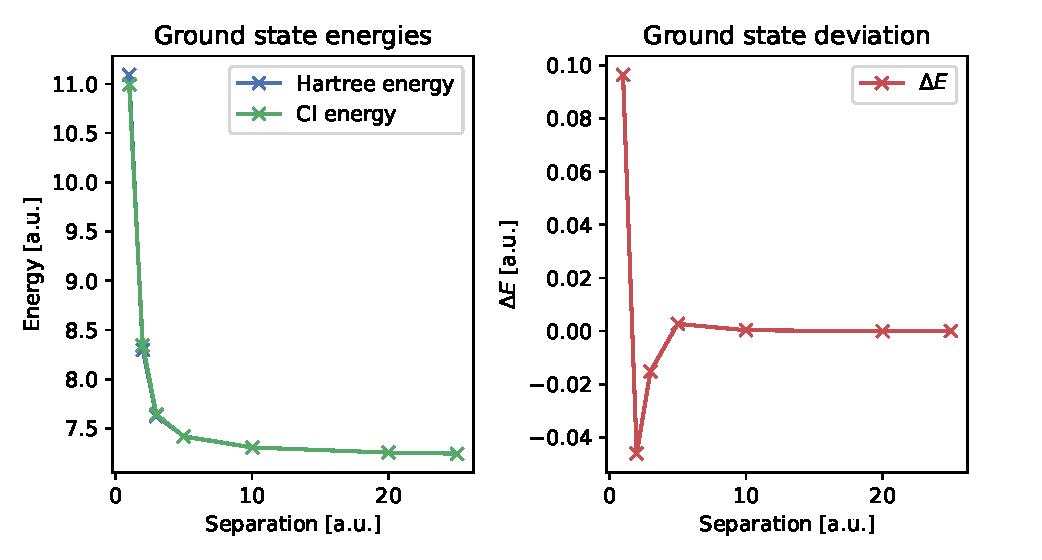
\includegraphics[width=1.0\textwidth]{figs/exchange_shift.pdf}
    \caption{Ground-state energy differenc $\Delta E = E_{HF} - E_{dist}$ as a function of the inter-well separation $d$ for the Morse double-well potential. The rapid decay of the energy shift with increasing well separation indicates that the exchange interaction has a negligible effect on the ground state energy, confirming our assumption of distinguishable particles in the system, and the reduced Hartree product-state converges to the full Hartree-Fock result even at moderate separations.}
    \label{fig:exchange_shift}
\end{figure}



\end{document}